\chapter{Software Project Management}

This chapter documents the project management artifacts for SHEO using the standard
project-management framework: the four~Ps, stakeholder analysis, Work Breakdown
Structure (WBS), effort estimation, scheduling, and risk management. These artifacts
reflect the actual scope and constraints of a small team building a software-only system.

% ---------------------------------------------------------------------------
\section{The Four Ps}
% ---------------------------------------------------------------------------

\subsection{People}
The development team consists of six developers, each taking on
overlapping roles across the project lifecycle.  No dedicated project manager
was appointed; instead, the team operated with shared responsibility and peer
review.  External stakeholders include the IoT contractor (Client), the building
management organisation (Customer), and the tenants who use the system daily
(End-users / Residents).  Skill coverage spans backend engineering (FastAPI,
Python), frontend development (React/JavaScript), systems integration, and
documentation.  The work was divided on a feature basis --- each member owns one
product module end to end, from its requirements through its design, code and tests.
Table~\ref{tab:task-alloc} records this allocation.

\begin{table}[htbp]
\centering
\caption{Team and task allocation. Each member owns one product module end to end.}
\label{tab:task-alloc}
\small
\begin{tabularx}{\linewidth}{@{}l l Y@{}}
\toprule
\textbf{Member} & \textbf{Student ID} & \textbf{Primary responsibility} \\
\midrule
Nguyen Tien Phat & 20235544 & Authentication, accounts and role-based access control; database schema and persistence; build, configuration and deployment. \emph{(Team lead / integration.)} \\
Chu Xuan Minh & 20235527 & Device monitoring and capability-driven control: real-time telemetry, the capability schema, command validation and offline detection. \\
Nguyen Dinh Truong & 20235566 & Explainable automation: the \texttt{WHEN--THEN} rule engine, conflict detection, the scheduler, and auto-actions with undo. \\
Vu Hai An & 20235468 & Habit recommendations and VND bill-saving estimation; the building-wide tariff model; reports and CSV export. \\
Nguyen Binh Anh & 20235470 & Frontend / UI--UX: all React pages, the capability-driven control widget, the live dashboard, and the usability evaluation. \\
Phung Gia Huy & 20235506 & Mock device simulator and live WebSocket streaming; the automated test suite and quality assurance (V-model, black-box and white-box testing). \\
\bottomrule
\end{tabularx}
\end{table}

\subsection{Product}
SHEO (AI-Driven Smart Home Energy Optimizer) is a web-based platform that
monitors household energy consumption through IoT device telemetry, supports
rule-based and AI-assisted device control, surfaces personalised energy-saving
recommendations, and estimates resulting cost savings.  The product scope is
bounded to a software application that communicates with a hardware abstraction
layer via a capability schema; no physical hardware is procured or modified.

\subsection{Process}
The team adopted an \emph{incremental} development approach: a functional
backend spine was delivered first, followed by successive increments adding
device control, the rules engine, the recommendation module, and the web UI.
Each increment closed with automated regression testing (67 test cases) and a
peer code-review pass.  This follows the Incremental model and
aligns with Agile values of working software and customer collaboration.

\subsection{Project}
The project is a temporary, unique endeavour with a fixed delivery date.
Key constraints are: no physical IoT hardware available (mitigated by a
deterministic simulator) and a six-person team with limited availability.  Success
is measured against the functional requirements (REQ-4.1--REQ-4.5), non-functional
requirements (NFR-PER, NFR-SAF, NFR-SEC), and the acceptance criteria in the test
plan.

% ---------------------------------------------------------------------------
\section{Stakeholder Analysis}
% ---------------------------------------------------------------------------

Table~\ref{tab:pm-stakeholders} identifies all stakeholders, their role,
and their principal interests and influence over the project.

\begin{table}[htbp]
  \caption{SHEO Stakeholder Analysis}
  \label{tab:pm-stakeholders}
  \centering
  \begin{tabularx}{\linewidth}{>{\bfseries}L{2.5cm} L{2.3cm} Y Y}
    \toprule
    Stakeholder & Role & Interest & Influence \\
    \midrule
    IoT Contractor
      & Client
      & Commission a reliable, extensible energy-management platform; protect investment in IoT hardware
      & High --- funds the project and defines the device capability schema \\
    \addlinespace
    Building Management / Apartment Owner
      & Customer (Administrator)
      & Reduce building-wide energy costs; maintain tenant satisfaction; oversee device onboarding and user accounts
      & High --- primary adopter; defines operational policy \\
    \addlinespace
    Resident (Tenant)
      & End-user
      & Convenient, safe device control; transparent energy feedback; actionable saving recommendations
      & Medium --- directly operates the system; acceptance drives adoption \\
    \addlinespace
    Development Team
      & Developer / Tester
      & Deliver a correct, maintainable product within project constraints
      & High (internal) --- executes all design, build, and test activities \\
    \addlinespace
    System Scheduler
      & Non-human actor
      & Execute time-triggered rules and telemetry aggregation reliably
      & Low (external input) --- a system component, not a human stakeholder \\
    \bottomrule
  \end{tabularx}
\end{table}

% ---------------------------------------------------------------------------
\section{Work Breakdown Structure}
% ---------------------------------------------------------------------------

Table~\ref{tab:wbs} decomposes SHEO into ten deliverable groups and their
constituent work packages.  Each leaf work package (WP) is assigned an
identifier, a brief description, and an acceptance criterion that can be
verified at handover.

\begin{longtable}{@{}p{0.6cm} p{3.8cm} p{7.6cm}@{}}
  \caption{SHEO Work Breakdown Structure with Acceptance Criteria}
  \label{tab:wbs} \\
  \toprule
  \textbf{WP} & \textbf{Work Package} & \textbf{Acceptance Criterion} \\
  \midrule
  \endfirsthead
  \toprule
  \textbf{WP} & \textbf{Work Package} & \textbf{Acceptance Criterion} \\
  \midrule
  \endhead
  \bottomrule
  \endlastfoot

  \multicolumn{3}{@{}l}{\textbf{1\ \ Monitoring}} \\[2pt]
  1.1 & Real-time dashboard
      & Dashboard displays live telemetry for all registered devices within 2~s of event receipt. \\[2pt]
  1.2 & Telemetry ingestion pipeline
      & Device readings are persisted to the database; simulator and live sources produce identical schema. \\[2pt]
  1.3 & Top-consumer identification
      & API returns the top-5 energy-consuming devices, ranked correctly, for any selected time window. \\[4pt]

  \multicolumn{3}{@{}l}{\textbf{2\ \ Device Control \& Capability Schema}} \\[2pt]
  2.1 & Capability schema registry
      & All device types expose a valid JSON capability document; unrecognised types are rejected at onboarding. \\[2pt]
  2.2 & Device command execution
      & Control commands update device state and are reflected in the UI within 1~s. \\[4pt]

  \multicolumn{3}{@{}l}{\textbf{3\ \ Rules Engine}} \\[2pt]
  3.1 & Rule authoring (CRUD)
      & Residents can create, read, update, and delete automation rules scoped to their own unit. \\[2pt]
  3.2 & Rule evaluation \& triggering
      & Time- and condition-based rules fire deterministically; conflicting rules are resolved by priority. \\[4pt]

  \multicolumn{3}{@{}l}{\textbf{4\ \ AI Recommendations (Habit Mining)}} \\[2pt]
  4.1 & Usage-pattern analysis
      & The recommendation engine produces at least one suggestion per device with 7~days of history. \\[2pt]
  4.2 & Recommendation lifecycle management
      & Residents can accept or dismiss recommendations; state transitions follow the documented FSM. \\[4pt]

  \multicolumn{3}{@{}l}{\textbf{5\ \ Savings Estimation}} \\[2pt]
  5.1 & Tariff model \& cost computation
      & Estimated monthly savings are within $\pm$5\% of a manually computed reference for the demo dataset; costs are stated in VND. \\[2pt]
  5.2 & Savings history \& reporting
      & Residents can view a 30-day savings trend with correct aggregation. \\[4pt]

  \multicolumn{3}{@{}l}{\textbf{6\ \ Web UI}} \\[2pt]
  6.1 & Resident portal
      & All Resident use cases (view, control, rules, recommendations) are reachable within 3 navigation steps. \\[2pt]
  6.2 & Administrator console
      & Administrators can onboard devices, manage accounts, and view building-wide analytics. \\[2pt]
  6.3 & Responsive layout \& accessibility
      & UI renders correctly at 1280~px and 375~px viewports; contrast ratio meets WCAG~AA. \\[4pt]

  \multicolumn{3}{@{}l}{\textbf{7\ \ Simulator \& Scheduler}} \\[2pt]
  7.1 & Deterministic device simulator
      & Simulator replays the seeded dataset identically on each run (fixed random seed). \\[2pt]
  7.2 & Background task scheduler
      & Scheduled rules fire at the configured time ($\pm$5~s); missed triggers are logged. \\[4pt]

  \multicolumn{3}{@{}l}{\textbf{8\ \ Authentication \& RBAC}} \\[2pt]
  8.1 & Token-based authentication
      & Login succeeds with valid credentials; invalid tokens are rejected as unauthenticated. \\[2pt]
  8.2 & Role-based access control
      & Resident endpoints are denied as unauthorised when accessed with an Administrator token and vice versa. \\[4pt]

  \multicolumn{3}{@{}l}{\textbf{9\ \ Testing}} \\[2pt]
  9.1 & Unit and integration test suite
      & Automated suite covers all REQ-4.x items; all 67 test cases pass on a clean checkout. \\[2pt]
  9.2 & Acceptance test mapping
      & Each functional requirement is traced to at least one passing test case in the test-plan RTM. \\[4pt]

  \multicolumn{3}{@{}l}{\textbf{10\ \ Documentation}} \\[2pt]
  10.1 & Software Requirements Specification
      & SRS is reviewed and signed off; all functional and non-functional requirements are enumerated. \\[2pt]
  10.2 & Software Design Document
      & SDD covers architecture, detailed design, UI/UX, and traceability; all diagrams are consistent with code. \\[2pt]
  10.3 & Project management report
      & This chapter is produced and included in the project documentation package. \\
\end{longtable}

% ---------------------------------------------------------------------------
\section{Effort Estimation}
% ---------------------------------------------------------------------------

Effort was estimated using a \emph{complexity-based sizing} method: each work
package was classified as Small (S), Medium (M), or Large (L) based on the number
of components involved, interface dependencies, and uncertainty.  A baseline
productivity rate was then applied (S~=~2~person-days, M~=~4~person-days,
L~=~7~person-days).  Table~\ref{tab:estimation} summarises the result.  Total
estimated effort is approximately \textbf{68 person-days} across the six-member
team over a twelve-week period (approximately 11~person-days per team member).

\begin{table}[htbp]
  \caption{Effort Estimation by Work Package}
  \label{tab:estimation}
  \centering
  \begin{tabularx}{\linewidth}{l X c c}
    \toprule
    \textbf{WP} & \textbf{Work Package} & \textbf{Complexity} & \textbf{Est.\ (person-days)} \\
    \midrule
    1   & Monitoring (dashboard + telemetry + top-consumers) & L & 7 \\
    2   & Device control \& capability schema               & M & 4 \\
    3   & Rules engine (CRUD + evaluation)                  & L & 7 \\
    4   & AI recommendations (habit mining + lifecycle)     & L & 7 \\
    5   & Savings estimation (tariff model + reporting)     & M & 4 \\
    6   & Web UI (Resident portal + Admin console + layout) & L & 7 \\
    7   & Simulator \& scheduler                            & M & 4 \\
    8   & Authentication \& RBAC                            & M & 4 \\
    9   & Testing (suite + acceptance mapping)              & L & 7 \\
    10  & Documentation (SRS + SDD + PM report)             & L & 7 \\
    \addlinespace
    --  & Integration, code review, and contingency (15\%) & -- & 10 \\
    \midrule
    \multicolumn{3}{r}{\textbf{Total estimated effort}} & \textbf{68} \\
    \bottomrule
  \end{tabularx}
\end{table}

\noindent
The integration and contingency buffer of approximately 15\% accounts for merge
conflicts, rework identified during peer review, and unforeseen dependencies
between the rules engine and the recommendation module.

% ---------------------------------------------------------------------------
\section{Project Scheduling}
% ---------------------------------------------------------------------------

\subsection{CPM Task Network}

Table~\ref{tab:cpm} lists the eight planning tasks, their predecessors, durations
(in calendar days), and the Early Start (ES) and Early Finish (EF) values computed
by the Critical Path Method.  All durations assume a parallel team of six with
partial time availability (estimated effective capacity of approximately 40\% per
day per member).

\begin{table}[htbp]
  \caption{CPM Task Schedule (calendar days from project start)}
  \label{tab:cpm}
  \centering
  \begin{tabularx}{\linewidth}{l X l c c c}
    \toprule
    \textbf{ID} & \textbf{Task} & \textbf{Predecessor(s)} & \textbf{Duration} & \textbf{ES} & \textbf{EF} \\
    \midrule
    T1 & Requirements analysis \& SRS        & ---         &  7 &  0 &  7 \\
    T2 & Architecture \& database design     & T1          & 10 &  7 & 17 \\
    T3 & Authentication \& RBAC              & T2          &  5 & 17 & 22 \\
    T4 & Device control \& capability schema & T3          &  8 & 22 & 30 \\
    T5 & Monitoring \& telemetry             & T4          & 10 & 30 & 40 \\
    T6 & Rules engine \& scheduler           & T4          & 12 & 30 & 42 \\
    T7 & Recommendations \& savings          & T5, T6      & 12 & 42 & 54 \\
    T8 & Web UI, testing \& documentation    & T7          & 14 & 54 & 68 \\
    \bottomrule
  \end{tabularx}
\end{table}

\noindent
The \textbf{critical path} is
T1~$\to$~T2~$\to$~T3~$\to$~T4~$\to$~T6~$\to$~T7~$\to$~T8,
with a total duration of \textbf{68 calendar days} (approximately 10~weeks).
Task~T5 (Monitoring) carries two days of float relative to T6 and is therefore
not on the critical path.

\subsection{Timeline Overview}

Figure~\ref{fig:gantt} provides a high-level Gantt-style view of the schedule.
Dark bars represent tasks on the critical path; the lighter bar represents the
non-critical Monitoring task (T5).

\begin{figure}[H]
  \centering
  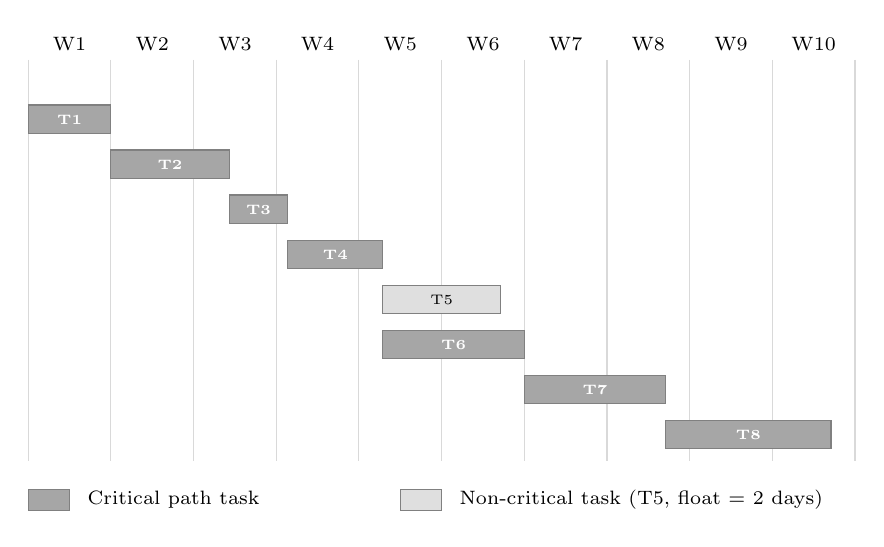
\begin{tikzpicture}[x=1.05cm, y=0.52cm]
    % Vertical grid lines at each week boundary
    \foreach \w in {0,...,10} {
      \draw[gray!30, thin] (\w, 0.3) -- (\w, -9.5);
    }
    % Week header labels
    \foreach \w in {1,...,10} {
      \node[above, font=\scriptsize] at (\w-0.5, 0.3) {W\w};
    }
    % Task bars (x-scale: 1 unit = 7 calendar days = 1 week)
    % T1: days 0-7  => x 0-1
    \filldraw[fill=gray!70, draw=black!50]
      (0,-0.8) rectangle (1,-1.5)
      node[midway, font=\tiny\bfseries, white] {T1};
    % T2: days 7-17 => x 1-2.43
    \filldraw[fill=gray!70, draw=black!50]
      (1,-1.9) rectangle (2.43,-2.6)
      node[midway, font=\tiny\bfseries, white] {T2};
    % T3: days 17-22 => x 2.43-3.14
    \filldraw[fill=gray!70, draw=black!50]
      (2.43,-3.0) rectangle (3.14,-3.7)
      node[midway, font=\tiny\bfseries, white] {T3};
    % T4: days 22-30 => x 3.14-4.29
    \filldraw[fill=gray!70, draw=black!50]
      (3.14,-4.1) rectangle (4.29,-4.8)
      node[midway, font=\tiny\bfseries, white] {T4};
    % T5: days 30-40 => x 4.29-5.71 (non-critical, float=2d)
    \filldraw[fill=gray!25, draw=black!50]
      (4.29,-5.2) rectangle (5.71,-5.9)
      node[midway, font=\tiny] {T5};
    % T6: days 30-42 => x 4.29-6.0 (critical)
    \filldraw[fill=gray!70, draw=black!50]
      (4.29,-6.3) rectangle (6.0,-7.0)
      node[midway, font=\tiny\bfseries, white] {T6};
    % T7: days 42-54 => x 6.0-7.71
    \filldraw[fill=gray!70, draw=black!50]
      (6.0,-7.4) rectangle (7.71,-8.1)
      node[midway, font=\tiny\bfseries, white] {T7};
    % T8: days 54-68 => x 7.71-9.71
    \filldraw[fill=gray!70, draw=black!50]
      (7.71,-8.5) rectangle (9.71,-9.2)
      node[midway, font=\tiny\bfseries, white] {T8};
    % Legend
    \filldraw[fill=gray!70, draw=black!50] (0,-10.2) rectangle (0.5,-10.7);
    \node[right, font=\scriptsize] at (0.6,-10.45) {Critical path task};
    \filldraw[fill=gray!25, draw=black!50] (4.5,-10.2) rectangle (5.0,-10.7);
    \node[right, font=\scriptsize] at (5.1,-10.45) {Non-critical task (T5, float = 2~days)};
  \end{tikzpicture}
  \caption{High-level project schedule (10-week view)}
  \label{fig:gantt}
\end{figure}

% ---------------------------------------------------------------------------
\section{Risk Management}
% ---------------------------------------------------------------------------

Risk management followed a five-step process: plan, identify, analyse
(Risk level~$=$~Probability~$\times$~Impact), respond
(Avoid / Transfer / Mitigate / Accept), and monitor.
Table~\ref{tab:risks} presents the SHEO risk register.
Probability is coded L~=~Low, M~=~Medium, H~=~High; impact is
Minor, Moderate, or Major.  The composite risk level is derived as
Probability~$\times$~Impact on a $3{\times}3$ ordinal scale
(L/M/H~$=$~1/2/3; Minor/Moderate/Major~$=$~1/2/3), giving integer values from~1
to~9.

\begin{longtable}{@{} p{2.5cm} p{1.4cm} p{0.7cm} p{1.4cm} p{0.7cm} p{1.5cm} p{4.3cm} @{}}
  \caption{SHEO Risk Register}
  \label{tab:risks} \\
  \toprule
  \textbf{Risk} & \textbf{Category} & \textbf{Prob.} & \textbf{Impact} & \textbf{Level} & \textbf{Response} & \textbf{Monitoring / Contingency} \\
  \midrule
  \endfirsthead
  \toprule
  \textbf{Risk} & \textbf{Category} & \textbf{Prob.} & \textbf{Impact} & \textbf{Level} & \textbf{Response} & \textbf{Monitoring / Contingency} \\
  \midrule
  \endhead
  \bottomrule
  \endlastfoot

  No physical IoT hardware available for development or demonstration
    & Technical
    & H
    & Major
    & 9
    & Mitigate
    & Replace with a deterministic software simulator (fixed seed); capability schema abstracts the hardware boundary so real devices can be integrated post-delivery without code changes. \\[4pt]

  Unsafe automatic actions on safety-critical devices (e.g., gas valves, fire suppression)
    & Safety
    & M
    & Major
    & 6
    & Mitigate
    & Automatic action is \emph{off by default} (NFR-SAF); the rules engine enforces a safety guard that prevents auto power-off of flagged devices; Residents must explicitly enable automation per device class. \\[4pt]

  Scope creep: feature additions beyond the agreed requirements baseline
    & Management
    & M
    & Moderate
    & 4
    & Mitigate
    & Requirements are frozen in the SRS after~T1; all change requests are impact-assessed before implementation; team reviews backlog scope at the start of each increment. \\[4pt]

  Tariff-model complexity: energy pricing structures vary by region and time-of-use period
    & Technical
    & M
    & Minor
    & 2
    & Accept / Mitigate
    & A simplified flat-rate and two-band time-of-use model is implemented; tariff parameters are externalised to a configuration file so Administrators can update rates in VND without code changes. \\[4pt]

  Demo non-reproducibility: randomised simulation produces different outputs on each run
    & Technical
    & H
    & Moderate
    & 6
    & Mitigate
    & All simulation components use a fixed random seed committed to the repository; the demo startup script re-applies the seed automatically, ensuring identical output on every execution. \\[4pt]

  Time and skills shortfall: team members lack experience with selected technologies
    & Management
    & M
    & Moderate
    & 4
    & Mitigate
    & The chosen web framework and client library are mature and widely adopted; a two-day spike was budgeted at~T2 for upskilling; pair programming is used on unfamiliar modules. \\[4pt]

  Cross-unit data leakage: a Resident accesses another unit's data via the API (IDOR)
    & Security
    & L
    & Major
    & 3
    & Mitigate
    & All resident-facing queries are scoped to the caller's own unit, while the Administrator's oversight queries deliberately span the building; an adversarial code-review pass specifically targeted cross-unit access vulnerabilities; all findings were corrected and re-tested before delivery. \\[4pt]

  Frontend--backend integration failure after independent parallel development
    & Technical
    & M
    & Moderate
    & 4
    & Mitigate
    & An interface contract is agreed and frozen at~T2, from which the front-end's typed access layer is generated; integration is exercised by the automated test suite from~T5 onward. \\

\end{longtable}

\noindent
The two highest-priority risks --- \emph{no physical hardware} (level~9) and
\emph{unsafe automatic actions} (level~6) --- are both mitigated by architectural
decisions embedded in the core design.  The remaining risks are re-evaluated at
the handover between each development increment.
